\documentclass{article}

\usepackage[small,compact]{titlesec}
\usepackage[backend=biber]{biblatex}
\usepackage[spanish]{babel}
\usepackage{epsfig}
\usepackage{array}
\usepackage{xfrac}
\usepackage{amsthm}
\usepackage{amsmath}
\usepackage{amssymb}
\usepackage{todonotes}
\usepackage{centernot}
\usepackage{textcomp}
\usepackage{blindtext}
\usepackage{centernot}
\usepackage{wasysym}
\usepackage{siunitx}
\usepackage[letterpaper]{geometry}
%\usepackage{multicol}
\usepackage{color}
%\usepackage[table]{xcolor}
\usepackage{amsfonts}
\usepackage{mathtools}
\usepackage{multirow}
\usepackage[small,it]{caption}
\usepackage{titling}
\usepackage{graphicx}
%\bibliographystyle{plain}
%\bibliographystyle{babplain}
\usepackage{filecontents}
\usepackage{titlesec}
\usepackage[section]{placeins}
\usepackage[hidelinks]{hyperref}
\usepackage{fancyhdr}
\usepackage{cancel}
\usepackage{abstract}
\usepackage{minted}

\sisetup{output-exponent-marker=\textsc{e}}

\captionsetup[table]{name=Tabla}


%\usepackage[makestderr=true]{pythontex}
%\restartpythontexsession{\thesection}

%\setpythontexoutputdir{./Temp}




\addbibresource{References.bib}

\pagestyle{fancy}
\usepackage[utf8]{inputenc}
\fancyhf{}
\fancyhead[c]{\textbf{\@title}}
\fancyfoot[c]{\thepage}
\def\Section {\S}

\newcommand\tstrut{\rule{0pt}{2.4ex}}
\newcommand\bstrut{\rule[-1.0ex]{0pt}{0pt}}

\DeclareMathOperator*{\argmax}{arg\,max}
\DeclareMathOperator*{\argmin}{arg\,min}

\setlength{\droptitle}{-4em}
\newcommand{\squishlist}{
 \begin{list}{$\bullet$}
  { \setlength{\itemsep}{0pt}
     \setlength{\parsep}{3pt}
     \setlength{\topsep}{3pt}
     \setlength{\partopsep}{0pt}
     \setlength{\leftmargin}{1.5em}
     \setlength{\labelwidth}{1em}
     \setlength{\labelsep}{0.5em} } }


\newcommand{\squishlisttwo}{
 \begin{list}{$\bullet$}
  { \setlength{\itemsep}{0pt}
    \setlength{\parsep}{0pt}
    \setlength{\topsep}{0pt}
    \setlength{\partopsep}{0pt}
    \setlength{\leftmargin}{2em}
    \setlength{\labelwidth}{1.5em}
    \setlength{\labelsep}{0.5em} } }

\newcommand{\squishend}{
  \end{list}  }
\footskip = 50pt
\setlength{\skip\footins}{10pt}

\newcounter{proofc}
\renewcommand\theproofc{(\arabic{proofc})}
\DeclareRobustCommand\stepproofc{\refstepcounter{proofc}\theproofc}
\newenvironment{twoproof}{\tabular{@{\stepproofc}c|l}}{\endtabular}

\usemintedstyle{tango}
 %% The usual stuff that sits
 %% between \documentclass
 %%    and \begin{document}

%\hypersetup{
%    bookmarks= \quadtrue,         % show bookmarks bar?
%    unicode= \quadfalse,          % non-Latin characters in Acrobat’s bookmarks
%    pdftoolbar= \quadtrue,        % show Acrobat’s toolbar?
%    pdfmenubar= \quadtrue,        % show Acrobat’s menu?
%    pdffitwindow= \quadfalse,     % window fit to page when opened
%    pdfstartview= \quad{FitH},    % fits the width of the page to the window
%    pdftitle= \quad{My title},    % title
%    pdfauthor= \quad{Author},     % author
%    pdfsubject= \quad{Subject},   % subject of the document
%    pdfcreator= \quad{Creator},   % creator of the document
%    pdfproducer= \quad{Producer}, % producer of the document
%    pdfkeywords= \quad{keyword1} {key2} {key3}, % list of keywords
%    pdfnewwindow= \quadtrue,      % links in new window
%    colorlinks= \quadfalse,       % false: boxed links; true: colored links
%    linkcolor= \quadred,          % color of internal links (change box color with linkbordercolor)
%    citecolor= \quadgreen,        % color of links to bibliography
%    filecolor= \quadmagenta,      % color of file links
%    urlcolor= \quadcyan           % color of external links
%}

%\addbibresource{References.bib}


\begin{document}
 %\thispagestyle{plain}
 \def\maketitle{%\twocolumn[%
 \thispagestyle{plain}
 \vspace{-10ex}
 \hrule
 \bigskip
 \begin{center}
 {\Large{\textbf{\@title}}}
 \end{center}
 \bigskip
 \hrule

 \bigskip

 \begin{flushleft}
 \textbf{\normalsize{Edgar Andr\'{e}s Margffoy Tuay}} \hfill 201412566
 \\
 \vspace{5pt}
 Universidad de los Andes \hfill Biomedical Engineering
 \\
 \vspace{5pt}
 Computer Vision \vspace{5pt}
\hfill \today \\ 
 \end{flushleft}
 %\hspace{265.2pt}
 }
\def\title#1{\def\@title{#1}}
\title{\textit{Hybrid Images}}



% \squishlist    %% \begin{itemize}
%\item First item
%%\item Second item
%%\squishend     %% \end{itemize}
 %% The rest of the paper (with no maketitle)
\maketitle

%\section{Diseño de filtros ideales}

%\begin{alignat}{2}
%h &= \begin{bmatrix}
%1 & 1 & 1 \\
%1 & 1 & 1 \\
%1 & 1 & 1 
%\end{bmatrix} \label{eq:e6}
%\end{alignat}


% \begin{equation}
% \begin{aligned}
% f ~:~ &\mathbb{R} &\longrightarrow ~ &\mathbb{R} \label{eq:e6} \\
%       &t &\longmapsto ~ &f(t)
% \end{aligned}
% \end{equation}
% \begin{equation}
% \begin{aligned}
% x ~:~ &\mathbb{Z} &\longrightarrow ~ &\mathbb{R} \label{eq:e7} \\
%       &n &\longmapsto ~ &x[n]
% \end{aligned}
% \end{equation}



% \begin{figure*}[!htbp]
% \centering
% \epsfig{file=./Assets/Discrete.pdf,width=1.0\linewidth,clip=}
% \caption{Ejemplos de señales discretas}
% \label{Fig:F3}
% \end{figure*}

\begin{abstract}
    Hybrid images is a method to merge two images, based on their frequency components and the biological process of image formation on the human eye, which disntiguishes low and higher frequency images based on the distance between the eye and the image, this approach allows to combine to images into one and trick the human eye to see one of the images when the composite is close, and the second image otherwise. 
\end{abstract}


\section{Introduction}
The perception process on the human eye is based on the composition of multiple frequency components and sprectrums according to the visual distance, that is, frequency components vary inversely with respect to distance, which means that higher frequencies are to be seen at lower distances and lower frequencies are associated to higher distances, this implies that is possible to form an image which presents different low and high frequency components coming from two different distributions, in this case, images (Hybrid Image).
\\
\\
To form an hybrid image, it is possible to process the input images ($x_1, x_2$) on the Fourier Frequency space and then extract their high and low frequency components by using Filters ($F_1, F_2$) (Low-pass and High-pass, respectively) \cite{Oliva:2006:HI:1141911.1141919}, after processing the images, it is possible to combine their responses in time to form a single image ($y$), it is necessary to observe that both input images must have the same dimensions\footnote{To get a consistent result it is possible to modify and set the cutoff frequencies and the kernel sizes defined for both filters.}. The process of hybrid image formation can be expressed as \eqref{eq:e1}

\begin{alignat}{2}
Y &= I_1 \cdot H_1 + I_2 \cdot (1 - F_2) \label{eq:e1}
\end{alignat}

\section{Materials and Methods}
To evaluate the feasibility of the procedure, an implementation was defined on Python, by using the OpenCV library to process basic Computer Vision operations, such as filter convolution and pyramid formation, Numpy was employed to manipulate image matrices and to apply operations in frequency domain, finally matplotlib was used to display and graph the results. To evaluate the synthesis method, different pair images were processed by using Gaussian Filters, designed in frequency domain and applied in time domain by using convolution, then to assess the final result a Gaussian Pyramid was built, it is expected that the high frequency components of the image can be seen on the first levels of the pyramid, but not in the last levels. With respect to the low frequency components, it is expected that the image can be seen on the last levels.


\section{Results}
After evaluating the method over different image pairs, it is possible to appreciate that the kernel size and the cutoff frequencies influence the result, for instance, if the cutoff frequency for the low pass filter is too high, the image may contain all the frequencies of the low-frequency image. Similarly, if the cutoff frequency for the high-pass filter is too low, then all the frequencies associated to the high-pass image may be reflected on the final result. With respect to the kernel size, it is possible to observe that increasing/decreasing the kernel size is equivalent to change the cutoff frequency. Additionally, to obtain consistent results, it is necessary that the images present similar geometry and pose orientations.
\\
\\
During the evaluation of the filters, it is possible to observe that applying the operations on the frequency space increases the memory consumption at the expense of the time complexity, especially if the images are large, for example to represent an image on frequency of dimension (6000, 4000, 3), it is necessary to use a space of dimension (6000, 4000, 2, 3), because the pixel intensities are transformed onto complex numbers. This implies that if the values are represented as floating numbers of 32 bits, then it is necessary to store 5.7Gb of data, compared to the computation time of a convolution in time with a lower memory footprint.

\section{Conclusions}
After evaluating the procedure to conform an Hybrid Image, it is possible to appreciate that different hyperparameters and geometry features of the input images can alter the final result, for instance, the cutoff frequencies and the kernel sizes of the filters implied on the process can atenuate or intensify the presence of the frequency components of the original images on the hybrid image. Also the procedure used to compute the final image may increase or decrease the memory footprint at the expense of the time complexity of the convolution operation, which means that the frequency/time tradeoff may be of interest when the dimensionality of the images change. Finally, synthetising hybrid images may be of interest on perception studies and art representations. 


 

%\bibliography{biblios} \nocite{*}
\nocite{*}
\printbibliography

\newpage
\section{Code Snippets}

\begin{listing}[H]
	\begin{minted}{python}
def pyramid_built_up(img, n):
    """
    Given an in imput image, build an image that contains n levels of the Gaussian Pyramid.

    Parameters
    ----------
    img: array_like
        Input image.
    n: int
        Number of pyramid levels to display.
    """
    composite = img
    last_lvl, cur_lvl = img, cv2.pyrDown(img)
    n -= 1
    for lvl in range(n):
       H, W, C = composite.shape
       mask = np.zeros((H, W + cur_lvl.shape[1], C))
       mask[-H:, 0:W] = composite
       mask[-cur_lvl.shape[0]:, W:W + cur_lvl.shape[1]] = cur_lvl
       composite = mask
       last_lvl, cur_lvl = cur_lvl, cv2.pyrDown(cur_lvl)
    return composite
	\end{minted}
	\caption{Function which builds an image that contains $n$ levels of the Gaussian Pyramid associated to an input image}
\end{listing}


\begin{listing}[H]
	\begin{minted}{python}
lp1 = butterworth(size_1, lp_freq, order) # Low pass frequency response
lp1_t = np.abs(fft.ifft2(lp1)) # Time domain representation
lp2 = butterworth(size_2, hp_freq, order) # High pass frequency response
lp2_t = np.abs(fft.ifft2(lp2)) # Time domain representation
\end{minted}
\caption{Declaration of high pass and low pass filters on frequency and time}
\end{listing}


\begin{listing}[H]
	\begin{minted}{python}

lp_img = cv2.GaussianBlur(img1, size_1, lp_freq) # Apply Gaussian filter (LP)
hp_img = img2 - cv2.GaussianBlur(img2, size_2, hp_freq) # Apply Gaussian filter (HP)

synth = lp_img + hp_img # Build Hybrid Image
\end{minted}
\caption{Filter convolution and image addition to conform Hybrid Image}
\end{listing}

\section*{Image results and Description}
\subsection*{Cold War}
\squishlist
\item \textbf{Description:} A mixture between Moscow Saint Basil Cathedral and New York City Statue of Liberty, these are good times for Humanity, isn't it?
\item \textbf{Processing:} Original images were of size (6016, 4000) and (4000, 6016) pixels, respectively. The images were cropped and centered.
\item \textbf{Parameters:} $\omega_{cl} = 0.1$, $\omega_{ch} = 21$, $|K_{l}| = 21 \times 21$, $|K_{h}| = 41 \times 41$
\item \textbf{Execution invocation:}
\squishend

\begin{minted}[breaklines]{bash}
python main.py  --lowpass 0.1 --highpass 21 --save output.jpg --lker_size 21 21 --hker_size 41 41 ./data/Moscow.jpg ./data/Liberty.jpg
\end{minted}

\begin{figure*}[!htbp]
	\centering
	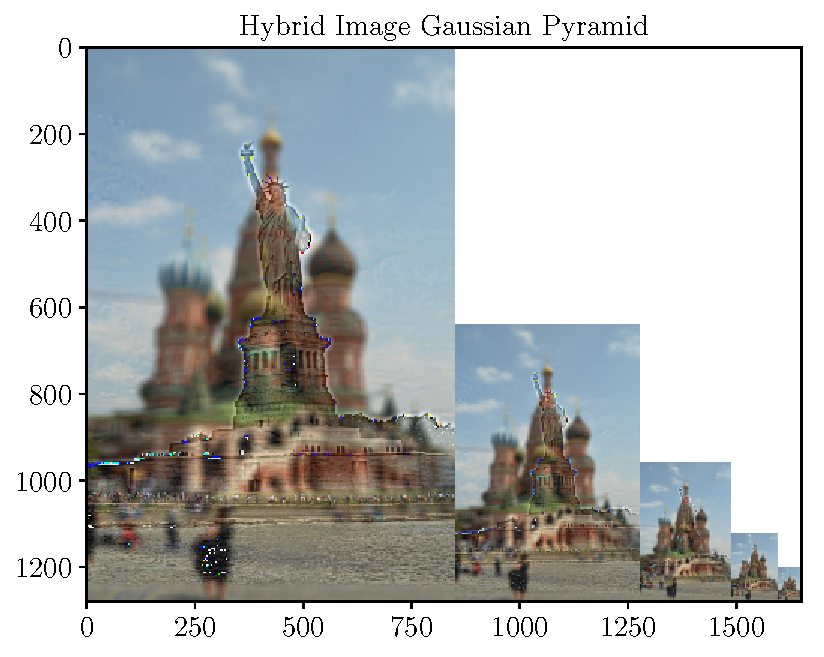
\epsfig{file=./Assets/pyr_Moscow_Liberty.pdf,width=0.6\linewidth,clip=}
	\caption{Gaussian Pyramid of level 5 \textit{Cold War} image}
	%\label{Fig:F1}
\end{figure*}


\begin{figure*}[!htbp]
	\centering
	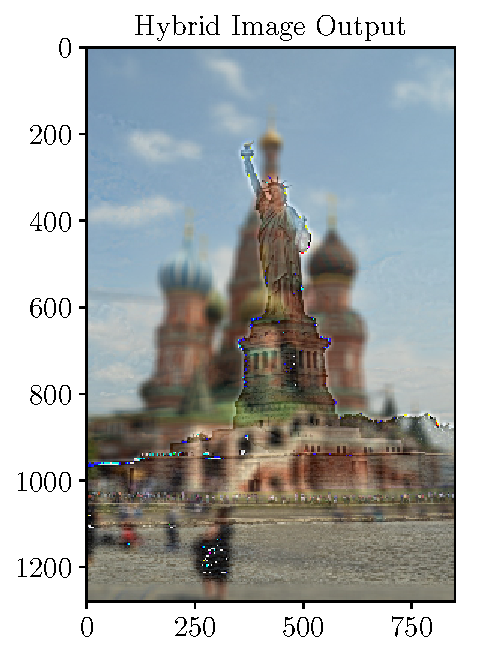
\epsfig{file=./Assets/result_Moscow_Liberty.pdf,width=0.5\linewidth,clip=}
	\caption{Hybrid image: \textit{Cold War} image}
	%\label{Fig:F1}
\end{figure*}

\subsection*{Two Face}
\squishlist
\item \textbf{Description:} Some friends decided to participate on this lab.
\item \textbf{Processing:} One of the images was cropped and translated
\item \textbf{Parameters:} $\omega_{cl} = 30$, $\omega_{ch} = 2$, $|K_{l}| = 11 \times 11$, $|K_{h}| = 3 \times 3$
\item \textbf{Execution invocation:}
\squishend

\begin{minted}[breaklines]{bash}
python main.py  --lowpass 30 --highpass 2 --save output.jpg --lker_size 11 11 --hker_size 3 3 ./data/Face_2.jpg ./data/Face_1.jpg 
\end{minted}

\begin{figure*}[!htbp]
	\centering
	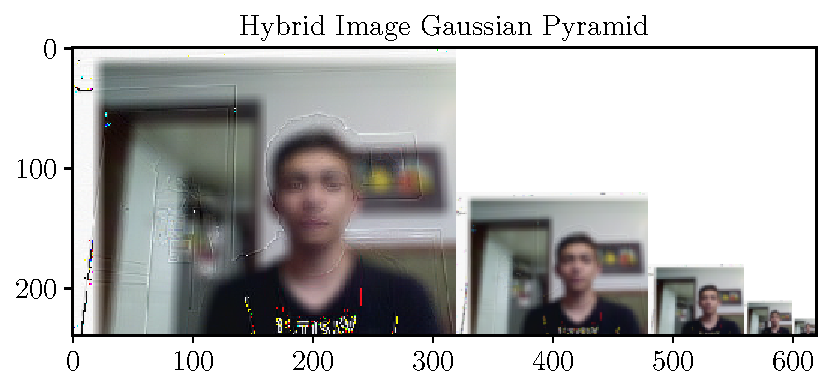
\epsfig{file=./Assets/pyr_Face_2_Face_1.pdf,width=0.8\linewidth,clip=}
	\caption{Gaussian Pyramid of level 5 \textit{Two Face} image}
	%\label{Fig:F1}
\end{figure*}


\begin{figure*}[!htbp]
	\centering
	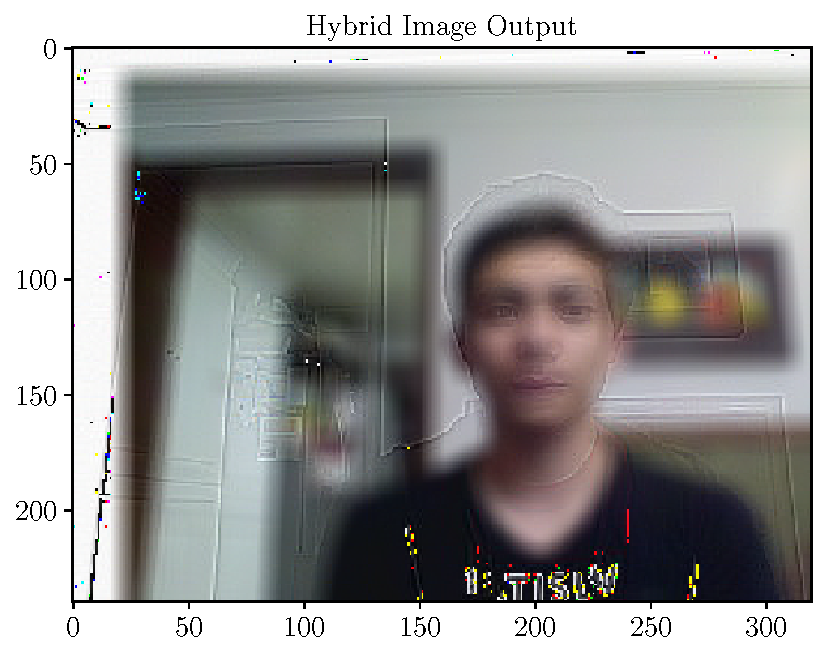
\epsfig{file=./Assets/result_Face_2_Face_1.pdf,width=0.8\linewidth,clip=}
	\caption{Hybrid image: \textit{Two Face} image}
	%\label{Fig:F1}
\end{figure*}


%\newcounter{proofc}
%\renewcommand\theproofc{(\arabic{proofc})}
%\DeclareRobustCommand\stepproofc{\refstepcounter{proofc}\theproofc}
%\newenvironment{twoproof}{\tabular{@{\stepproofc}c|l}}{\endtabular}


\end{document}